\section{Глубокие сближения, поверхность нулевой скорости и \(\xi\)-пространство}

Одной из ключевых задач исследования было понять, что происходит с орбитами при экстремально глубоких сближениях тел, и связаны ли эти сближения с какими-либо бифуркациями или с касанием границы области допустимого движения (поверхности нулевой скорости). В этом разделе показано, что наблюдаемые аномалии в спектре при \(d_{\min} \sim 10^{-10}\) являются артефактом точности, а не физикой, а поверхность нулевой скорости нигде не достигается.

\subsection{Разбор орбиты 1641: артефакт точности real128}
В блоке \textit{arclength} была найдена орбита с индексом \(idx=1641\), у которой минимальное расстояние между телами достигает \(d_{\min} = 1.97 \times 10^{-10}\), что на 5–8 порядков меньше, чем у остальных орбит семейства. При интегрировании в стандартной точности \texttt{real128} (\(\text{tol}=10^{-25}\)) для этой орбиты наблюдался спектр типа X2 (с двумя парами мультипликаторов, близких к \(+1\)) и аномально большое значение \(\max|\mu| = 32.7\), резко выделяющееся на фоне соседних орбит (\(\max|\mu| \approx 9.78\)).

Для выяснения природы этой аномалии были проведены систематические тесты:
\begin{enumerate}
    \item Переинтегрирование с точностью 64, 128, 192, 256 и 384 бита. Значение \(d_{\min}\) воспроизводится с точностью \(0.03\%\) на всех уровнях точности, то есть сближение реально.
    \item При \(\text{prec}=256\) (\(\text{tol}=10^{-60}\)) спектр меняется: вместо X2 наблюдается тип C с \(\max|\mu| = 9.78\), совпадающий с соседними орбитами 1640 и 1642.
    \item При \(\text{prec} \geq 256\) спектр воспроизводим и не зависит от \(\text{tol}\). При \(\text{real128}\) спектр оказался чувствительным к \(\text{tol}\) (значения 9.39, 48.8, 9.78 при \(\text{tol}=10^{-20}, \dots, 10^{-33}\)).
    \item Уточнение методом Ньютона сдвигает начальное состояние на \(\sim 10^{-12}\), а \(d_{\min}\) не меняется.
    \item Соседние орбиты 1640, 1642, 1620 при любых ограничениях метода Ньютона дают один и тот же \(d_{\min}\) и спектр.
\end{enumerate}
Вывод: \textbf{орбита 1641 не является бифуркацией}, а представляет собой артефакт точности \texttt{real128} при \(d_{\min} \sim 10^{-10}\). При повышении точности до 256 бит она ведёт себя как обычная орбита типа C. Геометрия 1641 — изоскелесная конфигурация с двумя одновременными сближениями пар (12 и 23 при \(t \approx 3.4105\); 12 и 13 при \(t \approx 6.9228\)).

\subsection{Геометрия \(\xi\)-пространства}
Для визуализации относительного движения и анализа поверхности нулевой скорости используется координатное пространство \(\xi = (\xi_1, \xi_2, \xi_3)\), введённое в разделе 2. В этих координатах:
\begin{itemize}
    \item точка равновесия \(\xi_{eq} = (-1, \sqrt{3}, 0)\);
    \item момент инерции \(I = |\xi|\);
    \item лучи коллизий (сближений пар тел 1–2, 2–3, 3–1) лежат в плоскости \((\xi_1, \xi_2)\) под углами \(\pi\), \(\pi/3\), \(-\pi/3\).
\end{itemize}
Траектории орбит в \(\xi\)-пространстве представляют собой замкнутые петли, проходящие вблизи \(\xi_{eq}\). 3D-визуализация траекторий (для нескольких репрезентативных орбит) показана на рисунке~\ref{fig:xi_space_3d}.

\begin{figure}[H]
    \centering
    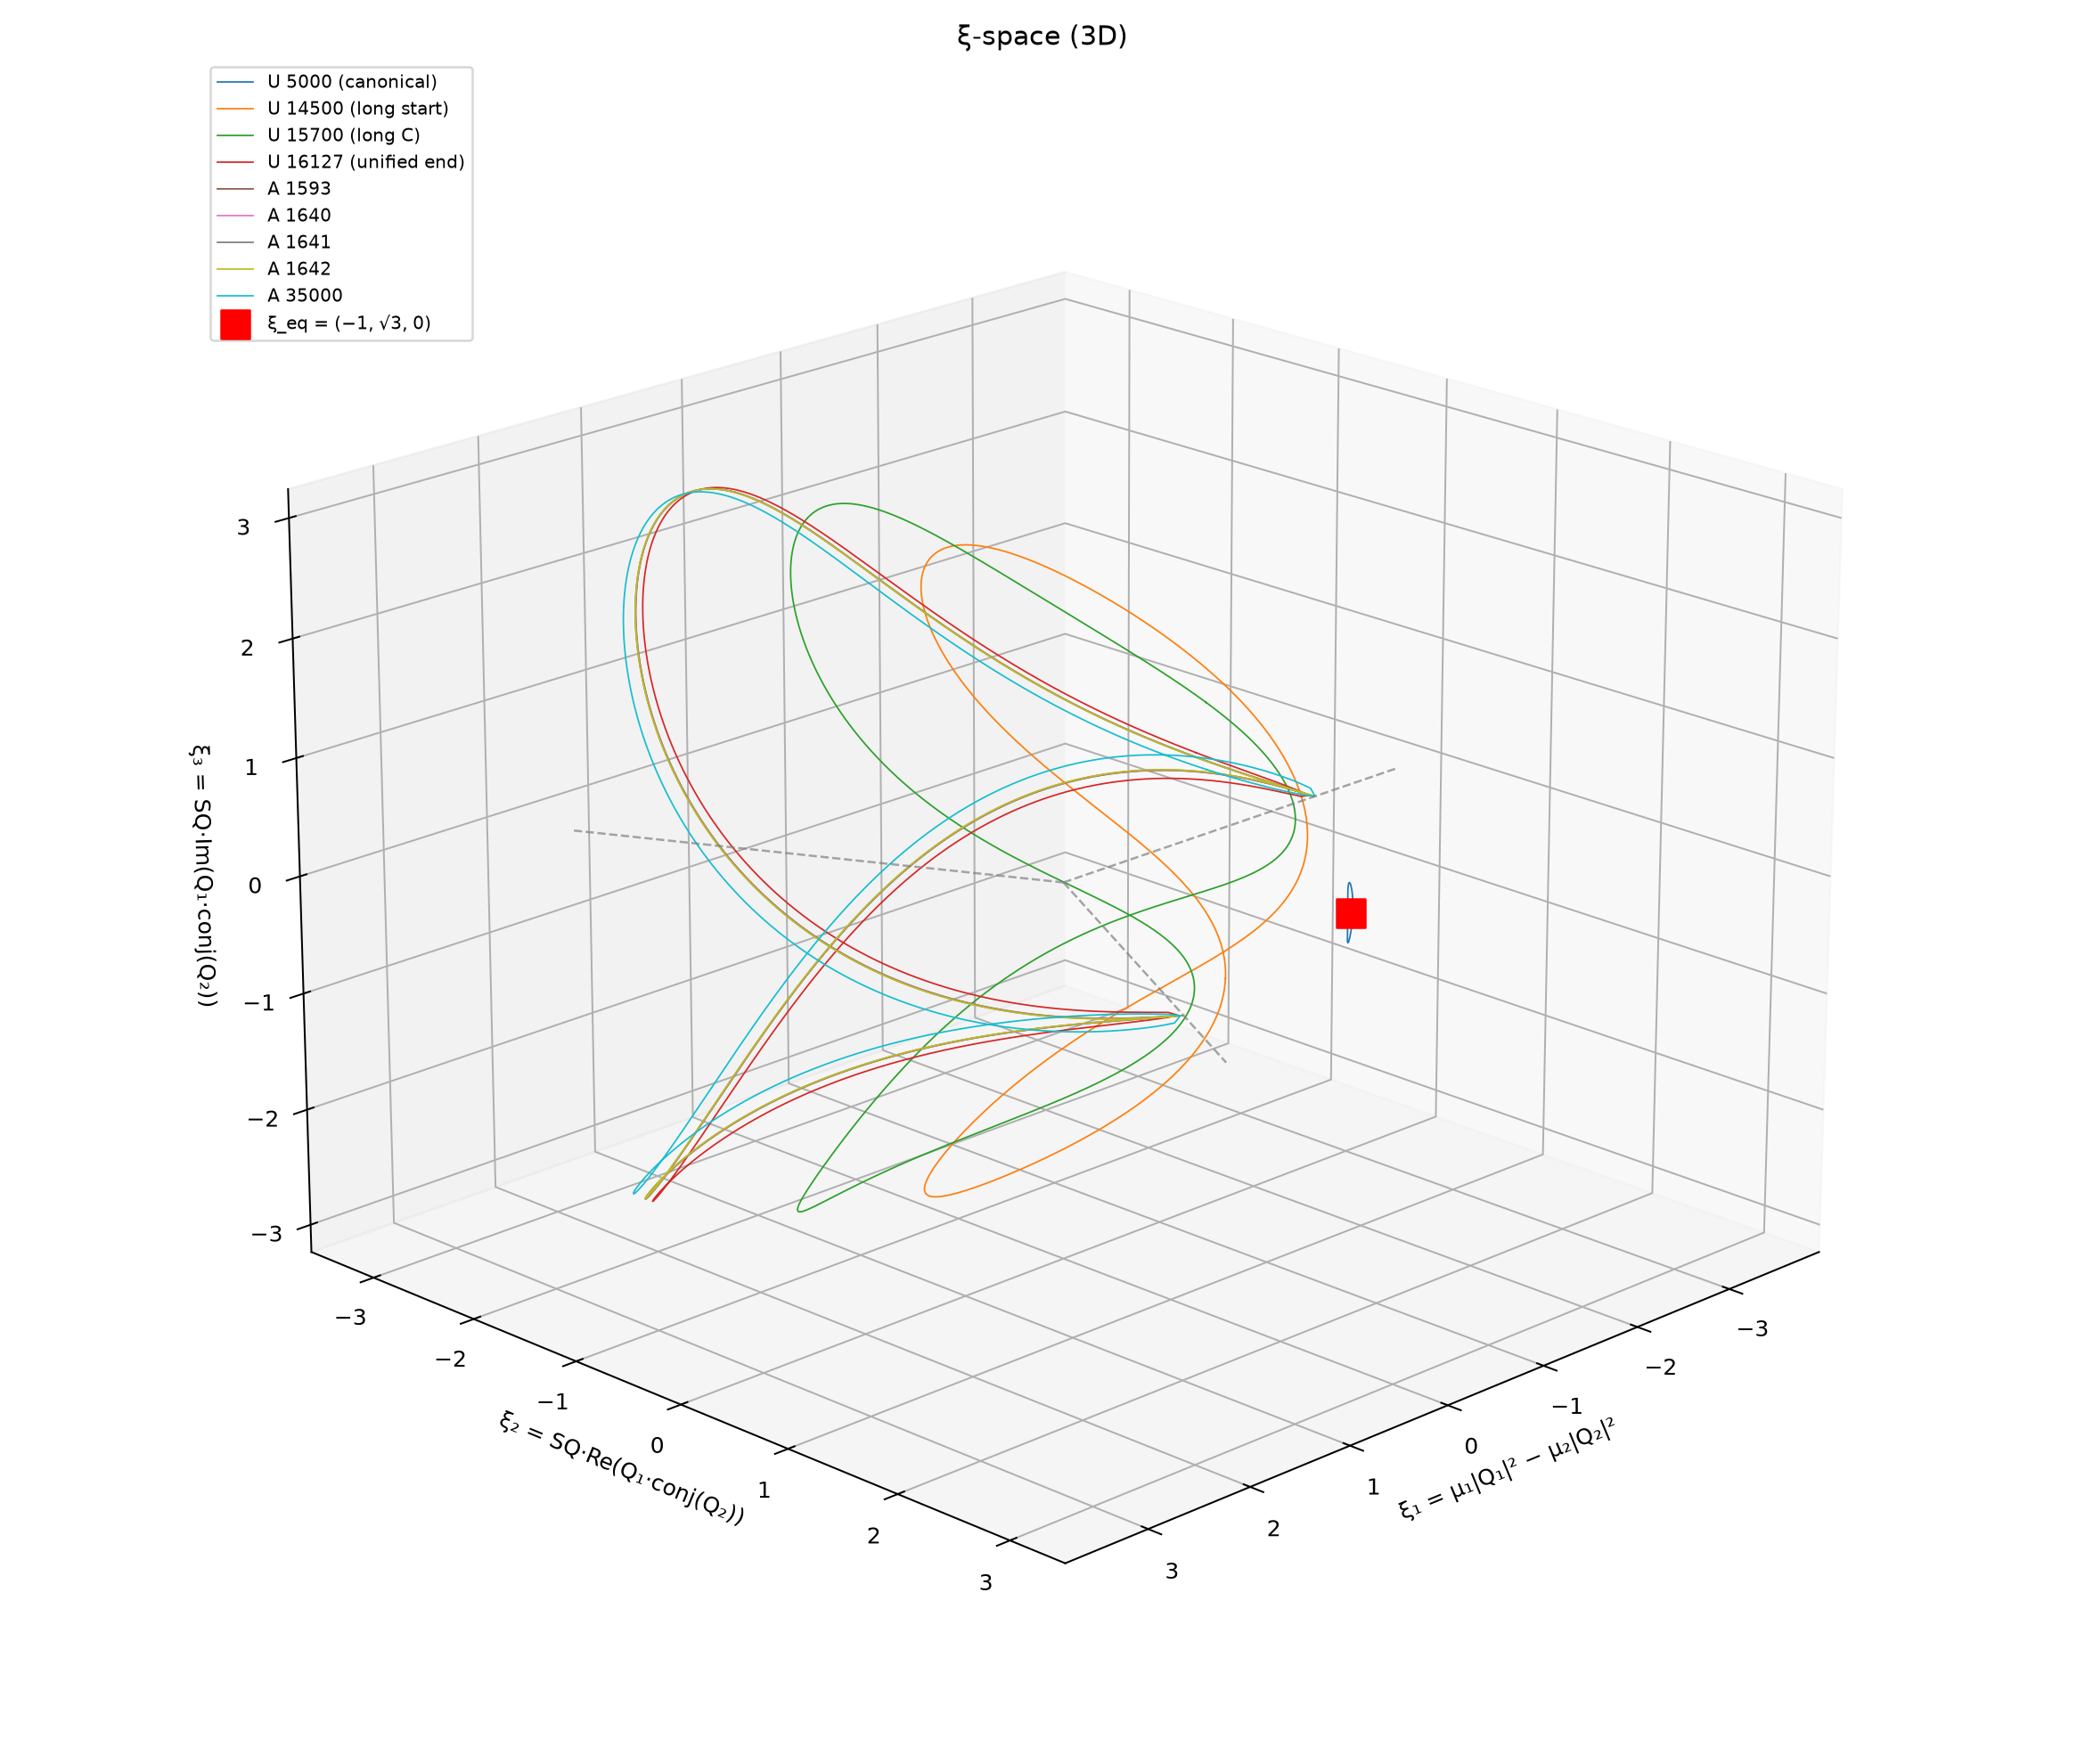
\includegraphics[width=0.85\textwidth]{93_xi_space_3d_v3.png}
    \caption{Траектории орбит в \(\xi\)-пространстве (3D). Точка \(\xi_{eq} = (-1, \sqrt{3}, 0)\) отмечена красным квадратом.}
    \label{fig:xi_space_3d}
\end{figure}

\subsection{Поверхность нулевой скорости в \(\xi\)-пространстве}
Поверхность нулевой скорости (ZVS) задаётся уравнением Сундмана (см. раздел 2):
\begin{equation}
    V(\xi) + \frac{L_z^2}{2|\xi|} = h_{in},
\end{equation}
где \(V(\xi)\) — потенциал, \(L_z\) — полный момент импульса в инерциальной системе, \(h_{in}\) — полная энергия в инерциальной системе. Область, где левая часть меньше \(h_{in}\), является доступной для движения; за её пределами движение невозможно.

Для всех орбит семейства \(h_{in} < 0\) (от \(-1.25\) в начале до \(-1.14\) в блоке \textit{arclength}), и \(h_{in}\) никогда не проходит через ноль. Это означает, что потенциал \(V(\xi)\) компенсируется центробежным членом \(L_z^2/(2|\xi|)\), и орбиты находятся в потенциальной яме, не касаясь границы.

На рисунке~\ref{fig:zvs_2d} показаны сечения ZVS в плоскости \(\xi_3 = 0\) для трёх репрезентативных орбит (A 1593, A 1641, U 16127). Чёрная линия — граница ZVS; зелёная область — доступная для движения; синяя линия — траектория. Видно, что \textbf{траектория всюду лежит в разрешённой области и не касается ZVS}.

\begin{figure}[H]
    \centering
    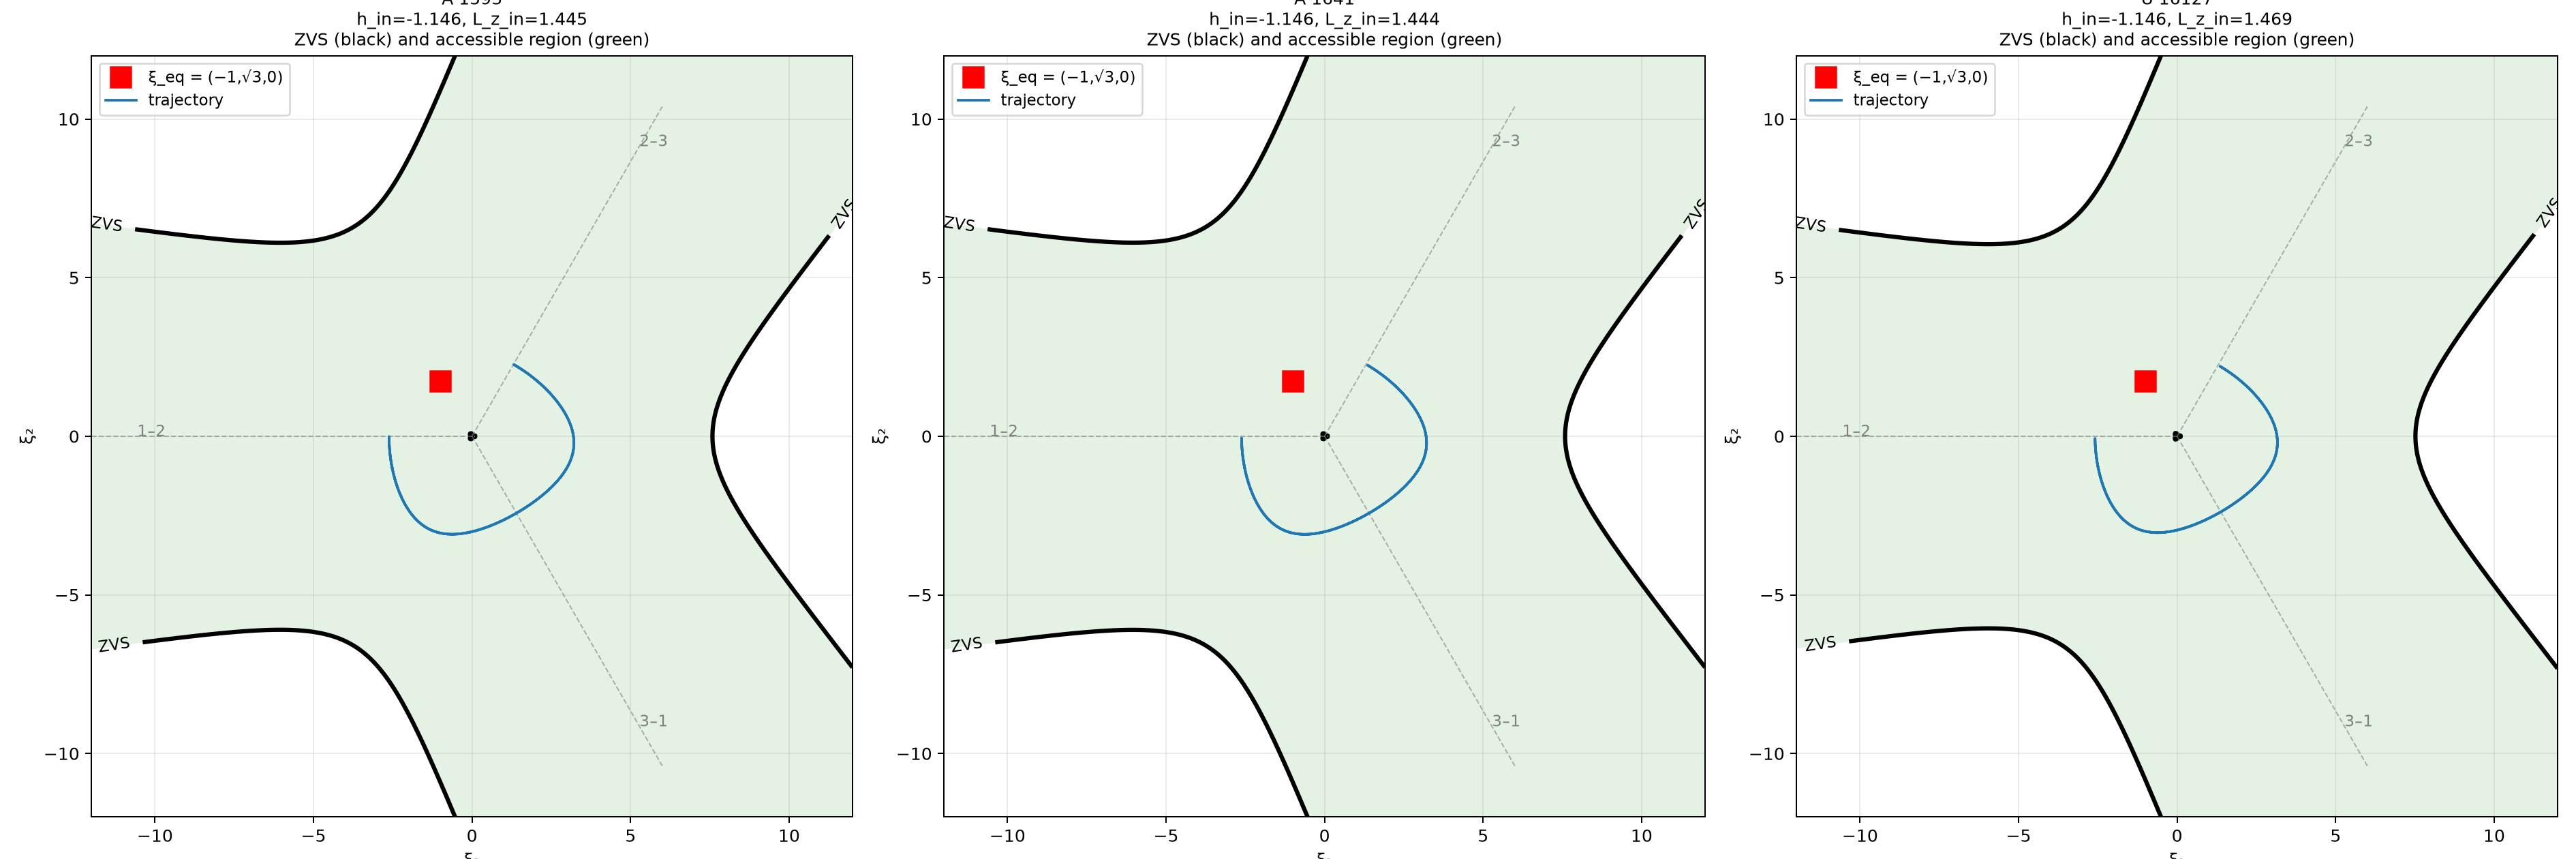
\includegraphics[width=\textwidth]{93_xi_zvs_xi3_0.png}
    \caption{Сечение поверхности нулевой скорости (ZVS) в плоскости \(\xi_3 = 0\) для трёх орбит (A 1593, A 1641, U 16127). Чёрная линия — ZVS; зелёным выделена доступная область; синяя линия — траектория орбиты. Лучи коллизий (пунктир) отмечены под углами \(\pi\), \(\pi/3\), \(-\pi/3\).}
    \label{fig:zvs_2d}
\end{figure}

3D-визуализация ZVS для орбиты A 1641 показана на рисунке~\ref{fig:zvs_3d}. Поверхность образует «капсулу» вокруг \(\xi_{eq}\), а «воронки», уходящие в бесконечность, соответствуют лучам столкновений (в них \(V \to -\infty\) и доступная область открывается). Траектория орбиты 1641 заключена внутри этой капсулы.

\begin{figure}[H]
    \centering
    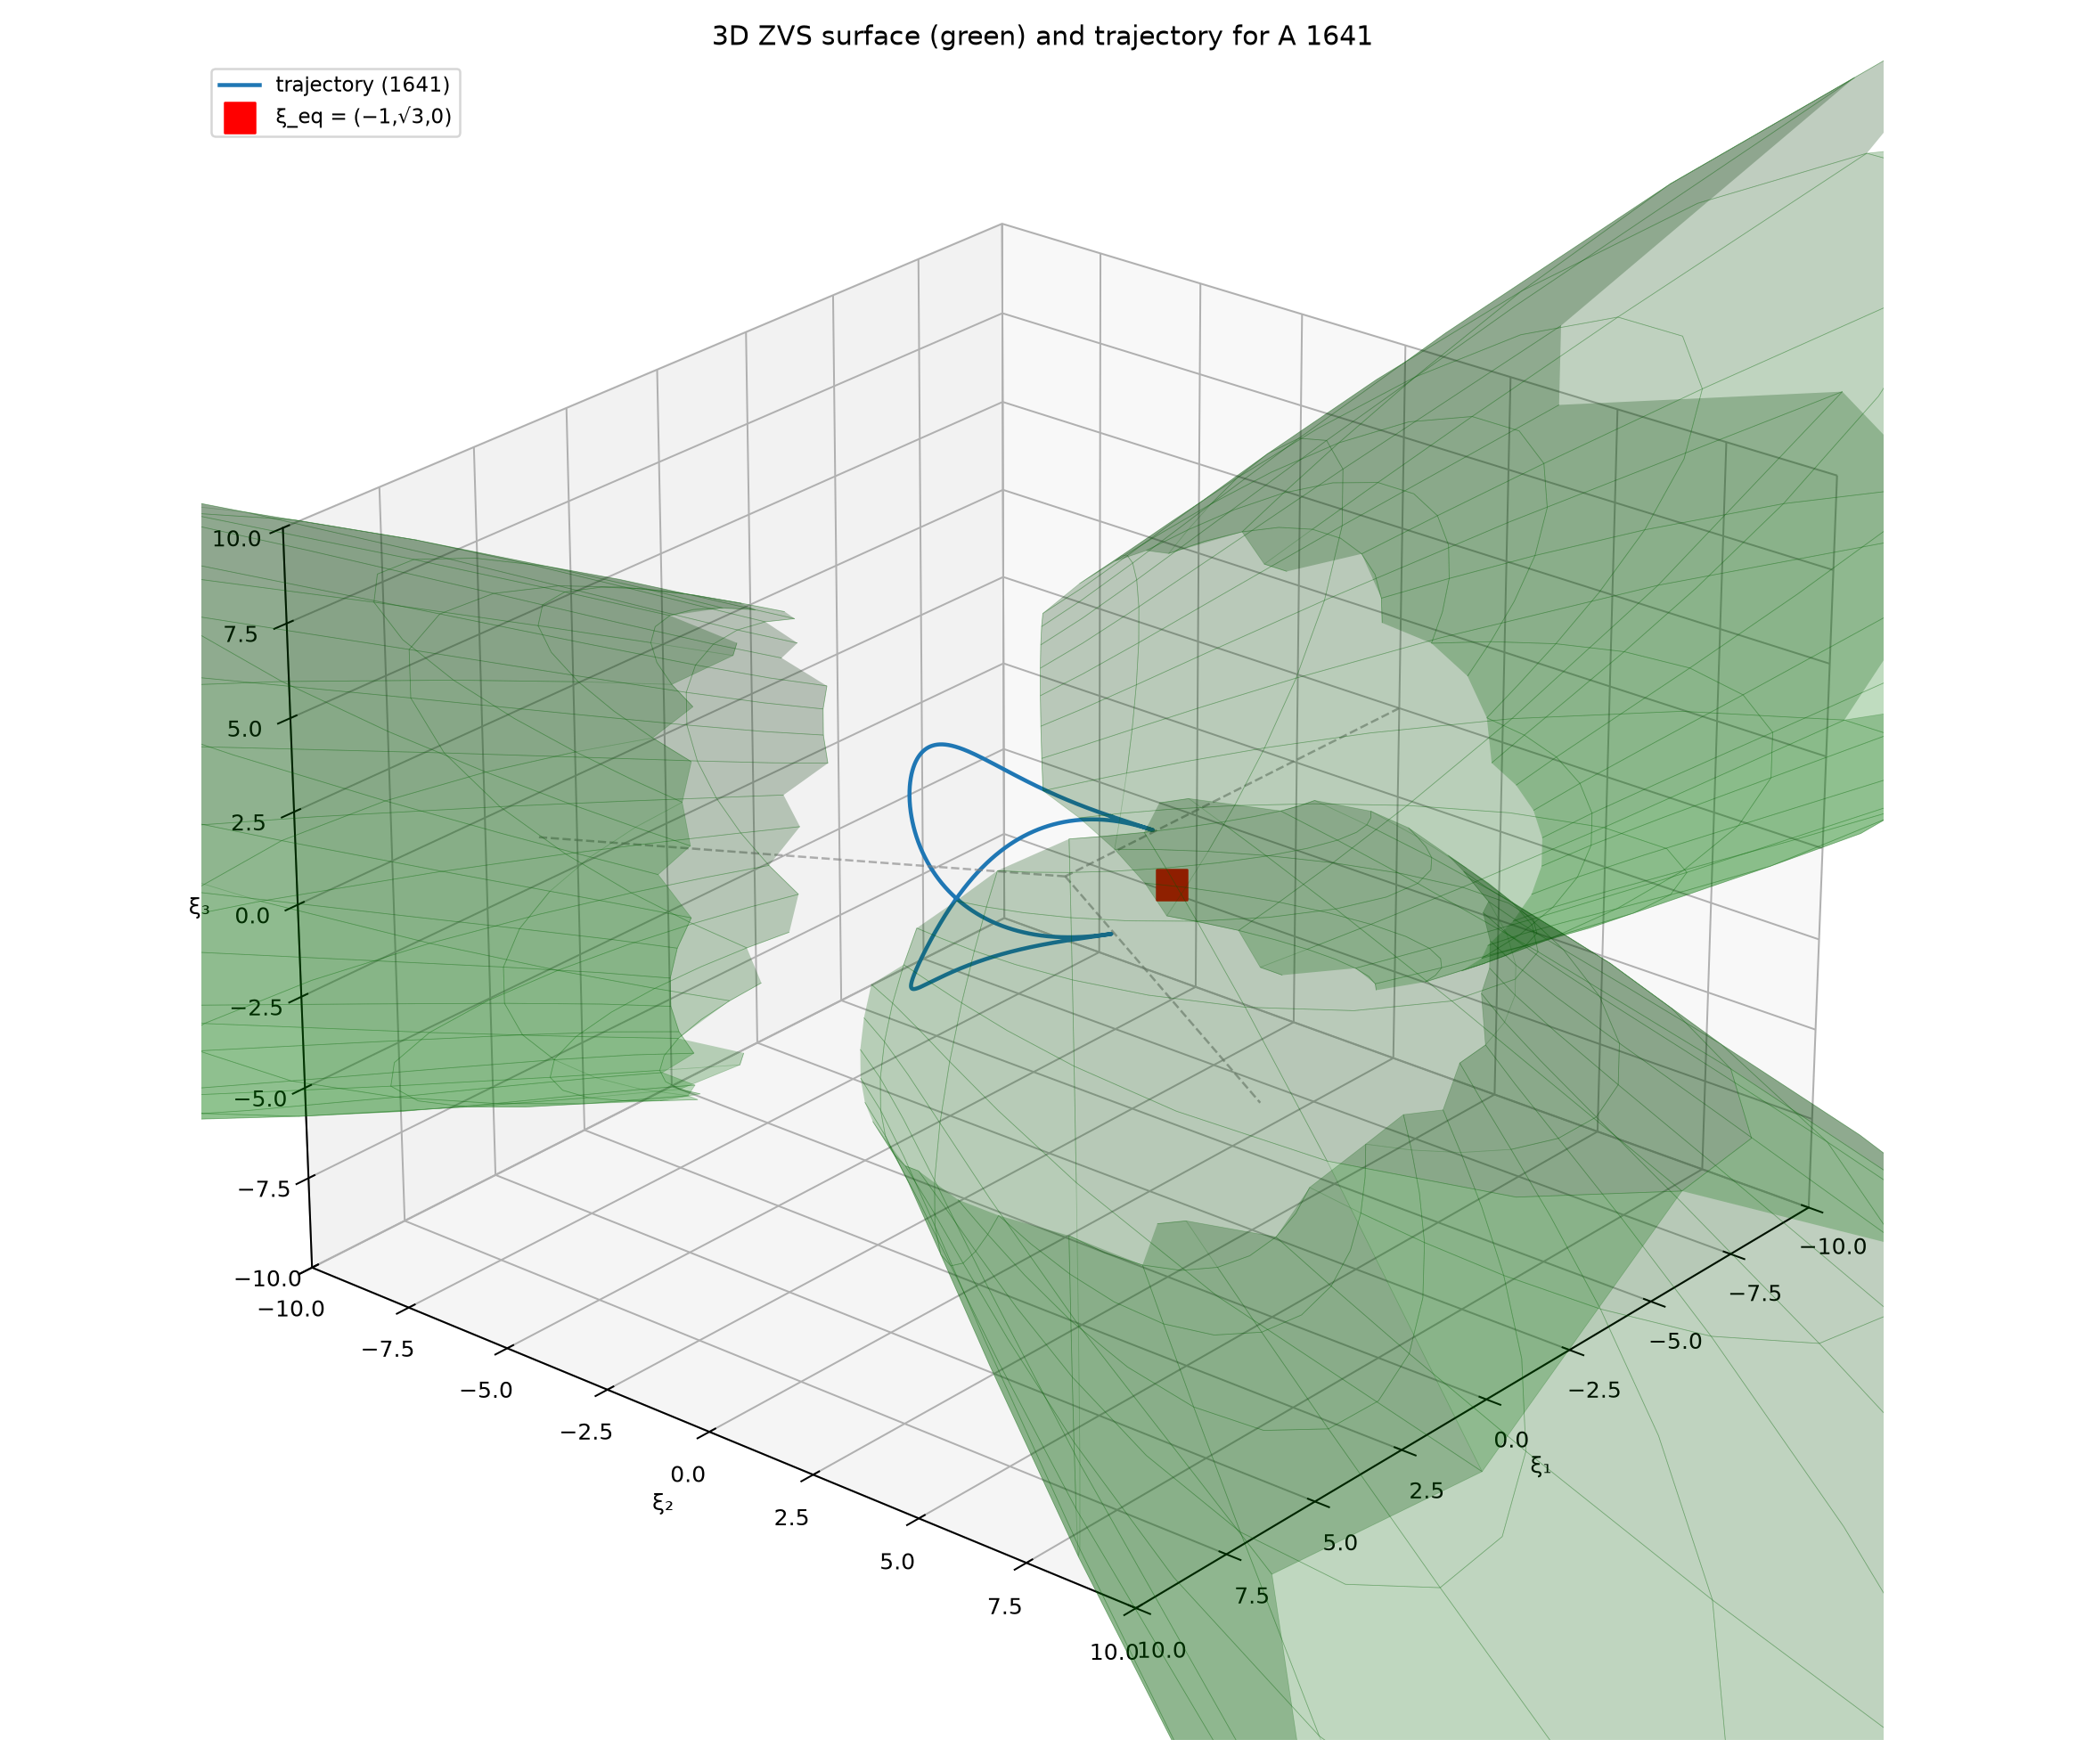
\includegraphics[width=0.85\textwidth]{93_xi_zvs_3d_1641.png}
    \caption{3D-визуализация поверхности нулевой скорости и траектории орбиты A 1641 в \(\xi\)-пространстве.}
    \label{fig:zvs_3d}
\end{figure}

\subsection{Запас по ZVS и отсутствие касания}
Количественно близость орбиты к ZVS характеризуется величиной
\begin{equation}
    \text{margin}(t) = h_{in} - V(\xi(t)) - \frac{L_z^2}{2|\xi(t)|},
\end{equation}
которая должна быть положительной для всех \(t\). Для всех проверенных орбит \(\min_t \text{margin}(t) > 0\) (обычно 1.5–2.4; минимальное значение \(\approx 1.1\) наблюдается около \(gidx \approx 15000\)). 

Графики \(\text{margin}(t)\) для трёх орбит (рисунок~\ref{fig:margin}) показывают, что запас положителен на всём периоде и имеет характерные пики в моменты сближений (там \(V\) резко возрастает по модулю, но не достигает \(h_{in}\)).

\begin{figure}[H]
    \centering
    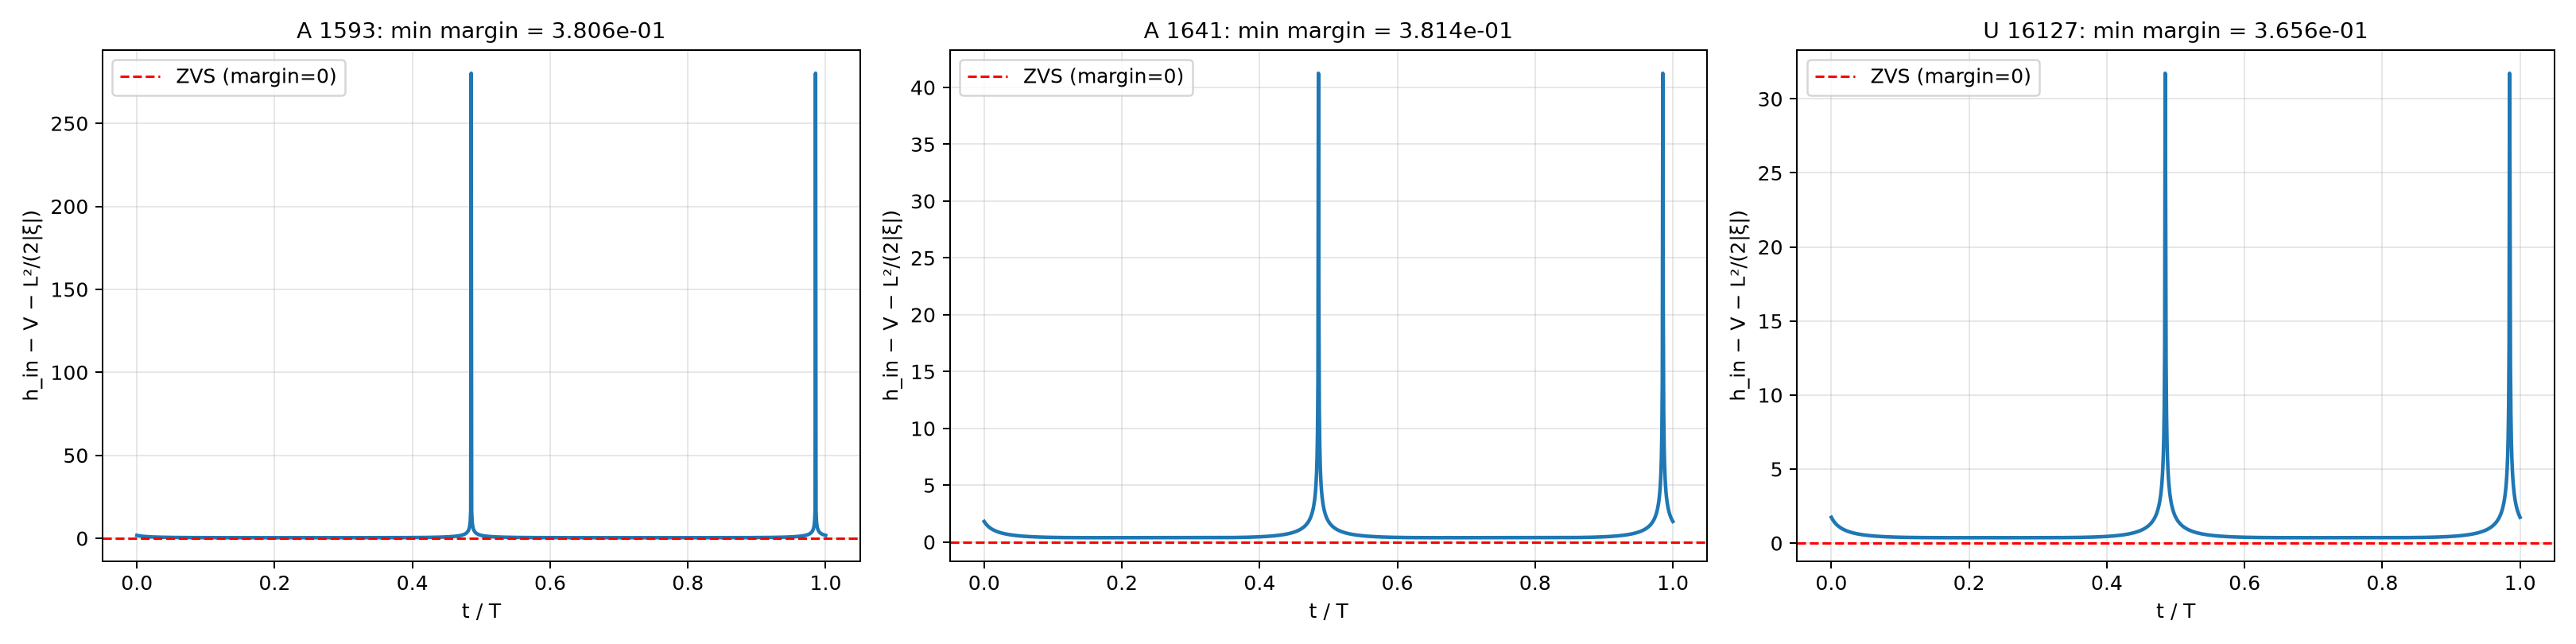
\includegraphics[width=\textwidth]{93_xi_margin.png}
    \caption{Запас \(\text{margin}(t) = h_{in} - V - L_z^2/(2|\xi|)\) вдоль траектории для трёх орбит. Красная линия — граница ZVS (\(\text{margin} = 0\)); она нигде не пересекается.}
    \label{fig:margin}
\end{figure}

\subsection{Вывод: ZVS не является механизмом переходов}
Совокупность результатов показывает: поверхность нулевой скорости \textbf{не является механизмом переходов} в этом семействе. Орбиты никогда не касаются ZVS, запас \(\text{margin}\) всюду положителен, а смена типа спектра (C \(\leftrightarrow\) R, OTHER \(\to\) C) происходит при значениях \(h_{in}\), далёких от критических. Ранее появлявшееся в скриптах сообщение о «переходе через ноль» было артефактом неверно заданных \(\xi_{eq}\) и углов коллизий, а также недостаточного сэмплирования.
